% arara: xelatex
% arara: xelatex
% arara: xelatex


% options:
% thesis=B bachelor's thesis
% thesis=M master's thesis
% czech thesis in Czech language
% english thesis in English language
% hidelinks remove colour boxes around hyperlinks

\documentclass[thesis=M,english]{FITthesis}[2012/10/20]

% \usepackage[utf8]{inputenc} % LaTeX source encoded as UTF-8
% \usepackage[latin2]{inputenc} % LaTeX source encoded as ISO-8859-2
% \usepackage[cp1250]{inputenc} % LaTeX source encoded as Windows-1250

\usepackage{graphicx} %graphics files inclusion
% \usepackage{subfig} %subfigures
\usepackage{amsmath} %advanced maths
% \usepackage{amssymb} %additional math symbols
\usepackage[]{algorithm2e}
\usepackage{xcolor}
\usepackage{float}
\newtheorem{problem}{Problem}

\usepackage{dirtree} %directory tree visualisation

% % list of acronyms
% \usepackage[acronym,nonumberlist,toc,numberedsection=autolabel]{glossaries}
% \iflanguage{czech}{\renewcommand*{\acronymname}{Seznam pou{\v z}it{\' y}ch zkratek}}{}
% \makeglossaries

% % % % % % % % % % % % % % % % % % % % % % % % % % % % % % 
% EDIT THIS
% % % % % % % % % % % % % % % % % % % % % % % % % % % % % % 

\department{Department of Theoretical Computer Science}
\title{Evaluating performance of an image compression scheme based on non-negative matrix factorization}
\authorGN{Marek} %author's given name/names
\authorFN{Pikna} %author's surname
\author{Marek Pikna} %author's name without academic degrees
\authorWithDegrees{Bc. Marek Pikna} %author's name with academic degrees
\supervisor{doc. Ing. Ivan Šimeček, Ph.D.}
\acknowledgements{THANKS (remove entirely in case you do not with to thank anyone)}
\abstractEN{Summarize the contents and contribution of your work in a few sentences in English language.}
\abstractCS{V n{\v e}kolika v{\v e}t{\' a}ch shr{\v n}te obsah a p{\v r}{\' i}nos t{\' e}to pr{\' a}ce v {\v c}esk{\' e}m jazyce.}
\placeForDeclarationOfAuthenticity{Prague}
\keywordsCS{Replace with comma-separated list of keywords in Czech.}
\keywordsEN{Replace with comma-separated list of keywords in English.}
\declarationOfAuthenticityOption{1} %select as appropriate, according to the desired license (integer 1-6)
% \website{http://site.example/thesis} %optional thesis URL

% dobry zdroje kompilace
% https://homepages.cae.wisc.edu/~ece533/project/f06/aguilera_rpt.pdf
% https://pdfs.semanticscholar.org/b481/96b92a6d28078b77f74f9129c3cd138ec291.pdf
% https://medium.com/@alfredayibonte/svd-and-image-compression-439c70745c99
% http://www.math.utah.edu/~goller/F15_M2270/BradyMathews_SVDImage.pdf
% https://www.mpi-inf.mpg.de/fileadmin/inf/d5/teaching/ss15_dmm/lectures/2015-05-26-intro-to-nmf.pdf - bozi prezentace
%     o praktickym nmf.
% https://eprints.soton.ac.uk/413094/1/NeuralComputationMDLPostReviews.pdf - volba ranku

% TODO
% Introduction - nejspise prepsat budouci cas na pritomny (tato cast je popsana, nikoliv bude popsana etc)
% Na konci introduction kde se popipisuji kapitoly asi prolinkovat jednotoliva cisla, jakmile budou.
% Prepsat v uvodu JPEG z algoritmu na format (+ png)
% TODO thesis na NMF - https://www.researchgate.net/profile/Ngoc_Diep_Ho/publication/262258846_Nonnegative_matrix_factorization_algorithms_and_applications/links/02e7e537226cb7e59b000000.pdf - excelentni stuff	
% TODO potencialne popsat, proc je potreba nezapornost (viz uvod vyse)
% TODO kapitola, ktera vysvetluje zaklady maticovyho poctu, co je to nonnegative matrix, matrix
%          multiplication a tak? kam s touhle kapitolou? podsekce v NMF sekci nebo vlastni kapitola?
%           zatim bych to napsal jako vlastni sekci, kdyztak se to presune
%           tam urcite - maticovy soucin, inverze, vektor * matice, transpozice matic
% TODO https://dial.uclouvain.be/pr/boreal/object/boreal:157009/datastream/PDF_01/view - zajimava vec o exaktnim NMF,
%      potencialne by byl gamechanger
% Prakticka cast - http://nimfa.biolab.si/nimfa.models.nmf.html - funkce sparseness() a estimate_rank().
% Prakticka cast - http://heather.cs.ucdavis.edu/NMFTutorial.pdf - choosing the rank SVD na obrazku!

% DULEZITE
% TODO - updatnout uvod (popsat co je teorie, co je uvod, odpovidajici kapitoly fixnout) - az bude vse
% TODO - presunout NMF jako treti kapitolu, kdyz tam ukazuju minimalni rank pro kompresi (a nerekl jsem, co je to komprese)
% TODO - Pripsat do digital image encoding, ze diskutujem jen rastry, vektorovy obrazky se tyhle prace netykaj
% TODO - Pridat do digital image encoding obrazek, kterej ukazuje pixely obrazku

% Moznosti nafouknuti
%   - Related work (nova kapitola)
%   - choice of rank r (nmf kapitola)
%   - nafouknuti matematickyho backgroundu (soucin matic a vse jine co je v NMF kapitole)
%   - color model vs color space (kapitola image encoding)

\begin{document}

% \newacronym{CVUT}{{\v C}VUT}{{\v C}esk{\' e} vysok{\' e} u{\v c}en{\' i} technick{\' e} v Praze}
% \newacronym{FIT}{FIT}{Fakulta informa{\v c}n{\' i}ch technologi{\' i}}

\setsecnumdepth{part}
\chapter{Introduction}
Data encoding and consequently data compression are both problems which lie
at the heart of many modern technologies - digital television, videogames, mobile
communications, security cameras and all other kinds of multimedia. As the amount
of data only grows in the current world, the quality of
compression ends up becoming a very serious problem, since good compression can
very significantly reduce the costs of data storage as well as the costs and speed
of data transfer.
\\

To put the problem into perspective, in order to store images in the resolutions
currently considered as high resolution (1920x1080 pixels, the second most common
resolution used on desktop devices \cite{res-stats}.
When storing an image with these dimensions using an uncompressed standard encoding,
the filesize would be almost 6 megabytes. Such a high size impacts many areas, such as
speed of transfer or storage costs. Fortunately, modern image compression formats such as
\emph{PNG} or \emph{JPEG} are able to reduce this size remarkably.
\\

Currently, images contribute to the amount of data on the internet significantly - not only are images a common
form of media for professional purposes but some of the currently largest platofrms on the
internet are based on image sharing and image hosting. One modern social media platform centered around image
sharing had over 67 million new posts each day \cite{data-amount}.
Being able to obtain these images fast and in good quality is therefore highly important for both users, just
as it is important for the owners of these services to be able to store this data.
\\

In the recent years with growht related to machine learning and similar areas, such as artifical
intelligence, new applications of mathematical concepts were discovered. Some of these concepts
which are enjoying high success are algorithms related to \emph{dimensionality reduction}. These
algorithms aim to reduce the number of random variables under consideration \cite{dimens-reduction}.
\\

While these algorithms have been enjoying success mostly in areas such as data mining or machine
learning, their nature of reducing the amount of random variables under inspection means that the
algorithms are essentially also compression algorithms. One of the algorithms used for dimensionality
reduction and the one which this thesis focuses on is \emph{non-negative matrix factorization} (abbreviated
as \emph{NMF}). The \emph{NMF} algorithm is currently used in areas such as facial recognition or
astronomy. Heart of the algorithm is the factorization of a matrix consisting of non-negative values into
matrices.
\\

The research in image compression methods using dimensionality reduction algorithms is currently being
performed - another dimensionality reduction algorithm and its potential usage for image compression 
which has been well researched is the \emph{singular value decomposition} algorithm, for example in \cite{svd-compression}. This algorithm, just like the \emph{NMF}, factorizes a matrix - however, without
restricting the values to be non-negative. While certain similar research to see whether
\emph{NMF} can be used for image compression exists, the works are related to very
specific use-case scenarios.
\\

Thus, this thesis aims to analyze the potential of the \emph{NMF} algorithm
as a tool for image compression. In order to achieve this, the following points
will be explored in the thesis:
\begin{itemize}
  \item \emph{NMF} and its current applications will be studied (Chapter~\ref{ch:NMF}).
  \item The theory and practice related to digital image encoding and image
        compression will be explored and described together with
        modern image compression . (Chapters~\ref{ch:image-encoding} and~\ref{ch:image-compression})
\end{itemize}

By analyzing these concepts, a proof of concept image compression algorithm using
\emph{NMF} will be designed and implemented. By doing so, these issues will be
addressed:
\begin{itemize}
  \item Whether a certain way of representing an uncompressed image is better
        suited for non-negative matrix factorization.
  \item Utilizing both subjective as well as objective metrics commonly used
        for evaluating quality of image compression, the performance of
        the proof of concept compression scheme will be evaluated.
  \item How well suited \emph{NMF} is for usage as an algorithm for image
        compression.
\end{itemize} 
At the end of the thesis, the proof of concept algorithm will be compared to
the state of the art image compression algorithms and possible points related
to further analysis or will be explored.
\\

The first three chapters are related to the theoretical part of the problem, studying
\emph{NMF}, image encoding and image compression. The following chapters are related
to the practical part of this thesis - design and implementation of the image
compression algorithm and its evaluation.

% Dale lze psat -
%   konkretni metody volby r - to by si zaslouzilo aspon trochu silnejsi popis a vysvetleni
%                              jednotlivych bodu
%   nmf a obrazkovou kompresi dal asi ne, to je vec casti navrhu nmf algoritmu
%   nimfu asi taky ne, ta bude v prakticky casti
%   rozepsat vic least squares
%   
\setsecnumdepth{all}
\chapter{Non-negative matrix factorization}
\label{ch:NMF}
This chapter discusses the \emph{non-negative matrix factorization} - defines
the problem, describes some of the existing solutions to the problem and
offers some observations. By doing so, the basics for the rest of the thesis are
provided.
\\

Non-negative matrix factorization as a problem was first formulated by Paatero
and Tapper in \cite{nmf-paatero}, but the works which have given
this problem far more popularity are the works of Lee and Seung \cite{lee99}, where
\emph{NMF} was applied to areas of machine learning and artificial
intelligence - more specifically to facial recognition and discovering semantic
features in encyclopedic articles.

\section{Problem definition}
Let $V$ be a $n \times p$ non-negative matrix, (i.e. with $x_{ij} \geq 0$, denoted
$X \geq 0$), and $r > 0$ an integer. Non-negative matrix factorization consists in
finding an approximation
\begin{equation}
  V \approx WH
\end{equation}
where $W, H$ are $n \times r$ and $r \times p$ non-negative matrices, respectively - meaning
all the elements of the matrices are non-negative.
In practice, the rank $r$ is often chosen such that $r \ll min(n,p)$. This is due
to the reason than in many common applications of non-negative matrix factorization,
the information contained in the matrix $V$ is summarized and split into $r$ factors
as the columns of $W$ \cite{nmf-r-vignette}.
\\

It should be noted here that the name of the problem might be misleading, as
the term \emph{"factorization"} is usually understood more as an exact
decomposition, whereas \emph{NMF} is in reality an approximation. Thus,
the problem is called \emph{non-negative matrix approximation} in certain
other works, such as \cite{nmf-approx}.

\section{Problem solution}
% TODO time complexity, standard algos, dulezitost volby r/max_iter?
In this section, two of the commonly used algorithms for solving the
non-negative matrix factorization problem will be described. The
first of these two algorithms will be the algorithm based on
\emph{multiplicative updates} as used in \cite{lee99}, where the
attention to part-based analysis, simplicity of the \emph{multiplicative
updates} and interpretability of the results helped to spread the influence
into many other research fields, such as image processing or text
processing \cite{nmf-phd-thesis}. Due to these reasons, this will be one of the algorithms
described. The second algorithm which will be described is the \emph{alternating
least squares} algorithm, which is the earliest algorithm proposed for solving
the non-negative matrix factorization problem (positive matrix factorization
in the original work) \cite{nmf-paatero}.
\\

The reason for choosing these two algorithms is that both of them are very
commonly used in practice. Other algorithms exist and are often researched,
example being the \emph{projected gradient} method \cite{projected-gradient}.
However, they will not be explored within this thesis.

\subsection{Multiplicative updates}
% TODO na zaver pripsat, ze velka sila je, jak je popsano v {lee-algos} v
%      jednoduchosti implementace.
The algorithm described here is described more thoroughly in \cite{lee-algos},
a work by Lee and Seung where the algorithms are described in detail together
with proving correctness of the algorithms.
\\

In order to find an approximate factorization $V \approx WH$, a way how to
quantify the quality of the approximation needs to be defined. Such a metric
(or a cost function) can be constructed by measuring the distance between
two non-negative matrices $A$ and $B$. One of the measures provided in
\cite{lee-algos} is the square of the Euclidean distance between $A$ and $B$.

\begin{equation}
||A - B||^2 = \sum_{ij}(A_{ij} - B_{ij})^2
\end{equation}

This distance is lower bounded by zero and vanishes if and only if $A = B$.
\\

By using this cost function, the non-negative matrix factorization can be
formulated as an optimization problem:
\begin{problem}
  Minimize $||V - WH||^2$ with respect to $W$ and $H$, subject to the constraints
$W, H \geq 0$.
\end{problem}
It is shown in \cite{lee-algos} that an algorithm cannot realistically solve this
problem by finding a global minimum. However, it is possible using various
techniques from numerical optimization which make it possible to find
local minimum.
\\

Thus, the multiplicative update rules are a compromise between speed and
ease of implementation offered in \cite{lee-algos} for solving this
problem. The multiplicative updates can be described as an algorithm below:
\\

\begin{algorithm}[H]
  \caption{Multiplicative update algorithm for NMF}
  \KwIn{Non-negative matrix V}
  \KwOut{Non-negative factors W and H}
  \begin{itemize}
    \item Initialize W and H as non-negative matrices\\
    \item Until $||V - WH||^2$ is minimized, update W and H by computing the
following, with n as an index of the iteration:\\
  \end{itemize}
  \begin{equation}
    H^{n+1}_{[i,j]} = H^{n}_{[i,j]} \frac{((W^{n})^TV)_{[i,j]}}{((W^{n})^{T}W^{n}H^{n})_{[i,j]}}
  \end{equation}
  and
  \begin{equation}
    W^{n+1}_{[i,j]} = W^{n}_{[i,j]} \frac{(V(H^{n+1})^{T}_{[i,j]}}{W^{n}H^{n+1}(H^{n+1})^{T}_{[i,j]}}
  \end{equation}
\end{algorithm}

It is shown in \cite{lee-algos} that the Euclidean distance $||V - WH||$ (and
consequently the cost function $||V - WH||^2$) is nonincreasing under these
rules. The work by Lee and Seung also considers another possible cost function and
proves the convergence of these rules.
\\

\subsection{Alternating least squares method}
Alternating least squares method is the first algorithm proposed for solving
the non-negative matrix factorization problem, which was proposed in the
work by Paatero. \cite{nmf-paatero} Fixing either of the factors $W$ or $H$,
the problem essentially becomes a least squares problem, which is commonly
used in \emph{regression analysis}.
\\

The alternating least squares problem then solves NMF using the algorithm
shown in \ref{alg:anls}.
\\

\begin{algorithm}[h]
  \caption{Basic Alternating least squares algorithm for NMF. \cite{nmf-anls}}
  \label{alg:anls}
  \KwIn{Non-negative matrix V}
  \KwOut{Non-negative factors W and H}
  \begin{itemize}
    \item Initialize W as random dense matrix\\
    \item Until a stopping condition:\\
    ~~\emph{(LS)} ~~~~~~~~~~Solve $min_{H \geq 0}||V - WH||^{2}$\\
    ~~\emph{(NONNEG)} Set all the negative elements of $H$ to $0$.\\
    ~~\emph{(LS)} ~~~~~~~~~~Solve $min_{W \geq 0}||V^{T} - H^{T}W^{T}||^{2}$\\
    ~~\emph{(NONNEG)} Set all the negative elements of $W$ to $0$.\\
  \end{itemize}
\end{algorithm}

As the least squares algorithm does not enforce the constraint of non-negativity,
all the negative elements in matrices are set to $0$ after each evaluation of
the least squares problem.
\\

The name of the algorithm reflects its nature where it keeps alternating between
solving the least squares problem for one fixed matrix and then the other.


\section{Common NMF applications}
% Duvod teto kapitoly - pozdeji take ukaze, ze pocet casti (napr. barevnych sloupcu)
% silne ovlivnuje kvalitu komprese - nebot vicemene provadim rozklad na tyto casti
In this section, a short example of a common application of non-negative matrix
factorizations will be provided, for the purpose of showing concrete examples
so that the reader may become more adjusted to the problem as well as showing
certain observations about the properties of non-negative matrix factorization.
\\


\subsection{Part-based analysis}
What has inspired the work of Lee and Seung \cite{lee99} was the human activity
of recognizing objects from basic parts - especially when using human vision which
is shown to be designed to detect the presence or absence of features (parts)
of physical objects in order to recognize them \cite{component-recognition}.
\\

Thus, assuming that features of an object would be independent and it would be
possible to compile all the features together, an object could be described
formally as:
\begin{equation}
  Object_{i} = Part_{1}(b_{i1})~\text{with}~Part_{2}(b_{i2})~\text{with...,}
\end{equation}
where $b_{ij}$ either has the value \emph{present} if part $i$ is present in object $j$ or
the value \emph{absent} if part $i$ is absent in object $j$.
\\

If the possible states \emph{present} and \emph{absent} in the model are
replaced by non-negative values, it is possible to signify not only the
presence or absence of a feature but also its quantity or significance
($b_{ij} \geq 0$). Thus, mathematically, a description of an object could
look like the following:

\begin{equation}
  Object_{i} = b_{i1} \times Part_{1} + b_{i2} \times Part_{2} + ...
\end{equation}\cite{nmf-phd-thesis}

When utilizing non-negative matrix factorization, the matrix $W$ can be
considered the set of features present in the data and matrix $H$ the set
of hidden variables. Non-negative matrix factorization can also be implemented
as:

\begin{equation}
  v_{i} \approx Wh_{i}
\end{equation}

Represented this way, the concept of non-negative matrix factorization can
be understood intuitively - each column in the original matrix $V$ is a data point.
Each column in the matrix $W$ is a basis element and columns of the matrix $H$ give the
coordinates of a data point in the basis $W$. The product matrix $WH$ (the approximation
of V) is a linear combination of the column vectors - the features extracted from
the data points and its significance in the data point.
\\

This way, features and parts can be extracted from
the original data and understood, as shown in the next subsection on the
image learning example.


\subsection{Image learning}
Digital image processing is a field which is currently enjoying high
popularity when it comes to research. Image processing is the field thanks
to which it is possible to extract features from images or recognize
various patterns. Principal component analysis \emph{(PCA)} is a dimensionality
reduction technique similar to \emph{NMF} commonly used for recognizing
faces in images \cite{pca-facial} - however, without the non-negativity constraint.
It has been shown in \cite{lee99} that \emph{NMF} can be used in a similar
fashion while potentially classifying the data in a way which is easier to be understood.
\\

\begin{figure}[h]
  \centering
  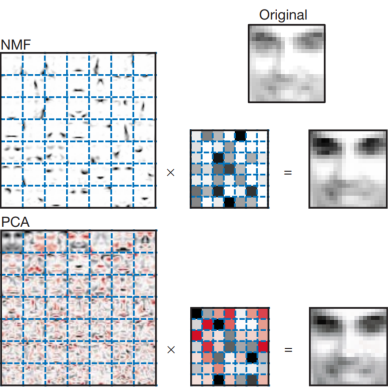
\includegraphics{nmfpca-comparison}
  \caption{Comparison between dimensionality reduction algorithms - \emph{NMF} and \emph{PCA},
           as shown in \cite{lee99}.}
  \label{fig:nmfpca-comparison}
\end{figure}

The Figure \ref{fig:nmfpca-comparison} has been taken from \cite{lee99}, where a database of
2,429 facial images has been taken and used to create a matrix $V$. By
applying both \emph{NMF} as well as \emph{PCA} to the matrix, feature
and coeffiecient matrices were created and particular instance of a
face was approximately represented by a linear superposition of basis
images. The coefficients used in the linear superposition are shown in the
montages, where black pixels indicate positive values and red pixels indicate
negative values. It can be seen on these montages that while \emph{NMF}
can be used for the same purposes as \emph{PCA}, the main strength of the
algorithm is that certain parts can be recognized meaningfully - for example
parts of a nose and such, whereas in the case of \emph{PCA}, discovering
meaning in the matrices is difficult.
\\

It is for these reasons that non-negativity is a powerful and meaningful
constraint, as parts are never subtracted from the particular instance
(as it can happen in the case of \emph{PCA}), but are only added together \cite{nmf-phd-thesis}.
\\


\subsection{NMF properties}
Previous sections in this chapter have described non-negative matrix factorization,
more specifically the definition of the problem, common solutions and an example
usage of \emph{NMF}. In this section, certain properties of non-negative matrix
factorization will be pointed out. When the proof of concept image compression scheme
is designed, the usefulness of these properties for compression will be discussed.
\\

The first property which will be shown is that the solution to non-negative matrix
factorization is \textbf{not unique}. A matrix and its inverse can transform the two
factorization matrices, for example as:
\begin{equation}
  V \approx WH = WBB^{-1}H
\end{equation}

If the matrices $\bar{W} = WB$ and $\bar{H} = B^{-1}H$ are non-negative then they
form another solution to the \emph{NMF} problem.\cite{nmf-nonuniq}
\\

Another important property is that the non-negative matrix factorization is not
hierarchical, meaning that the factor matrices using rank $r$ can be completely
different to those of rank $r+1$, as shown in \ref{fig:nmf-hierarchy}, where choice of
rank $r = 1$ provides only approximation of the target matrix $V$ yet rank $r = 2$ makes it
possible to calculate $V = WH$ instead of the approximation. Due to these
reasons, the results provided by using \emph{NMF} highly depend on choice of the rank
parameter.
\\

\begin{figure}[h]
  \centering
  \caption{Visual display of non-hierarchical properties of NMF. \cite{nonhierarchy}}
  \label{fig:nmf-hierarchy}
  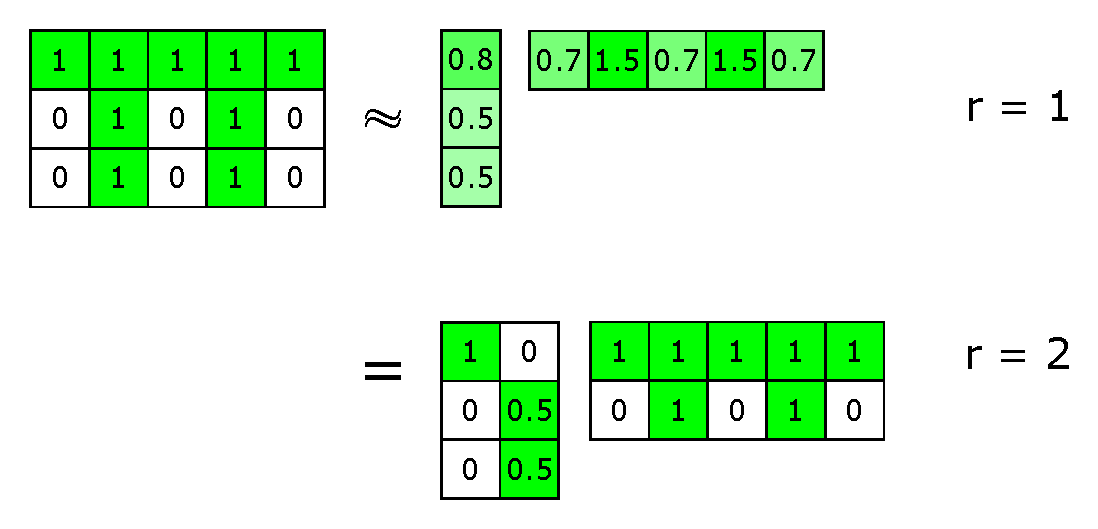
\includegraphics[scale=0.7]{non-hierarchical}
\end{figure}

However, one of the most important properties to note is that non-negative matrix
factorization is very difficult to solve and the existing general algorithms
solve \emph{NMF} as an optimization problem. Not only that but it has even been
proven that non-negative matrix factorization is an \emph{NP-hard} problem.\cite{nmf-nphard}
With certain constraints, it is however possible to solve the \emph{NMF} problem
in polynomial time - for example it is shown in \cite{nmf-poly} that in case the
matrix $V$ is symmetric and contains a diagonal principal submatrix of rank $r$,
it is possible to solve the problem in polynomial time $O(rm^{2})$.
\\

The last property of non-negative matrix factorization to be noted has been
shown in the figures above. The factors extracted are often \emph{sparse} - it is
precisely for this reason that interpreting results of non-negative matrix
factorization is easy in fields such as image processing or text mining (but many
others as well).\cite{nmf-whyhow}

\subsection{Choice of rank $r$}
The choice of rank $r$ is one of the most important problems when utilizing non-negative
matrix factorization - as when used for the examples above, choice of rank $r$
changes the amount of features to be extracted in order to approximate the target
matrix $V$.
\\


There are several common methods used for choosing the rank $r$:
\begin{itemize}
  \item Trial and error - try different values of \emph{r} and choose the one
        performing the best for application at hand.
  \item Estimate the rank $r$ using various statistical approaches (such as by
        using \emph{SVD}).
  \item The use of expert insights.
\end{itemize}\cite{nmf-whyhow}


\section{NMF and compression}
% TODO popsani rozmeru matic, r = n/2 vypocet, treba i obrazek...
Most common use-case scenarios of non-negative matrix factorization are
related to machine learning, as shown in the previous sections. However,
\emph{NMF} can also be looked upon as a lossy compression tool (more
on lossy compression in chapter \ref{ch:image-compression}), as an
original matrix of size $n \times p$ is approximated by the product
of two smaller matrices. Assuming the target matrix $V$ is represented
in the same way as the factor matrices $W$ and $H$, if the amount
of elements contained in matrices $W$ and $H$ is lower than the amount of
elements in matrix $V$, then \emph{NMF} was used to perform compression.
\\

Whether the amount of elements in factor matrices $W$ and $H$ is lower than
the amount of elements in target matrix $V$ depends on the choice of rank $r$.
More specifically, if the dimensions of matrix $V$ are $n \times p$, the
dimensions of matrix $W$ $n \times r$ and the dimensions of matrix $H$
$r \times p$, then this requirement can be formalized as:
\begin{align*}
  n \times r + r \times p &< n \times p\\
  r (n + p) &< n \times p\\
  r &< \frac{n \times p}{n + p}
\end{align*}

Considering a square matrix ($n = p$), the following relationship can also
be deduced:
\begin{align*}
  r &< \frac{n \times n}{n + n}\\
  r &< \frac{n^{2}}{2n}\\
  r &< \frac{n}{2}
\end{align*}
This relationship is also demonstrated in the figure \ref{fig:maxrank}.

\begin{figure}[h]
  \centering
  \caption{Visualization of NMF as a compression tool. When using a rank $r$ lower than $n/2$, the
           total amount of elements in matrices $W$ and $H$ is less than the amount of elements in
           matrix $V$. When the rank $r$ reaches the value $n/2$, the amount of elements is the same.}
  \label{fig:maxrank}
  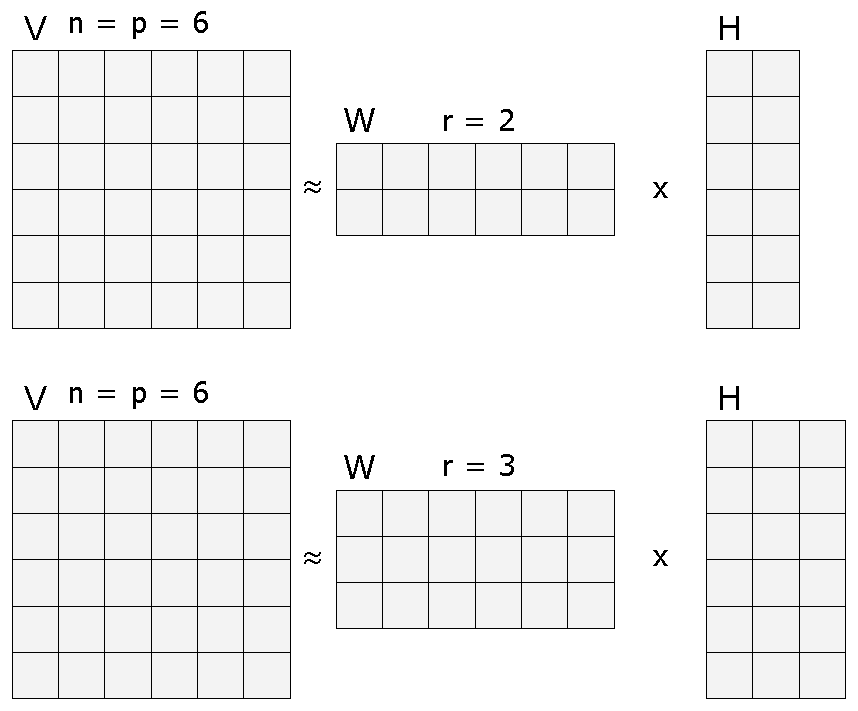
\includegraphics[scale=0.7]{maxrank}
\end{figure}

% [TODO]
%\section{Other types of NMF}
%Nice to have, ale nyni neni priorita.


% [TODO] mozna pripsat rozdil mezi color modelem a color spacem
\chapter{Digital image encoding}
\label{ch:image-encoding}
The second chapter of this thesis is related to digital images and their
representations color models. The importance of this chapter is related to
creating the image compression scheme and its empirical testing on
various different digital image representations. The possible ways of
specifying colors in digital images which will be explored are \emph{RGB},
\emph{grayscale} and $Y'C_BC_R$. As this thesis is related to image
compression and non-negative matrix factorization and not image processing,
only the most important elements of image encoding and color spaces will be explored.


% TODO http://apachetechnology.in/ati/www/KC/dw/Saloman%20-%20Data_Compression_Complete_Reference.pdf
%  `sampling and quantization str 253
\section{Digital images}
% http://elib.mi.sanu.ac.rs/files/journals/ncd/12/ncd12017.pdf
% https://www.spacetelescope.org/static/projects/fits_liberator/image_processing.pdf
% http://www.imageprocessingplace.com/downloads_V3/root_downloads/tutorials/Image%20Processing%20Fundamentals--An%20Overview.pdf - ideal
% https://www.researchgate.net/figure/A-digital-image-is-a-2D-array-of-pixels-Each-pixel-is-characterised-by-its-x-y_fig1_221918148
A digital image $I$ is stored as a matrix of \emph{pixels} (abbreviation for a \emph{picture
element}). These matrices described as 2D discrete space are derived from analog
images in 2D continuous space through the process called \emph{sampling}. More about
sampling can be found for example in \cite{img:img-processing}.
\\

The value assigned to a pixel $I[m,n]$ determines its color. The following sections
explore the common color encoding options.


\section{Color models}
A color model is a mathematical model used for describing the way of representing
colors, usually as tuples of numbers (although this is not necessary, as in i.e.
the \emph{grayscale} model). When associated with a description of how the tuple
components are interpreted, colors can be interpreted. The color models described
are the \emph{RGB} color model, the $Y'C_{B}C_{R}$ color space (the set of colors
which can be used) which is a transformation using the \emph{RGB} model and the
\emph{grayscale} model.


% https://www.spacetelescope.org/static/projects/fits_liberator/image_processing.pdf
\subsection{RGB}
The \emph{RGB} color model is closely related to the way the human eye perceives colors
with the \emph{r} (red), \emph{g} (green) and \emph{b} (blue) receptors in our retinas.\cite{img:color-theory}
In order to represent a color, components of each color (red, green and blue) are added together.
As these components are added together, the \emph{RGB} model is considered to be an additive one.
\\

In order to store image data using the \emph{RGB} color model, the color components
need to be quantified. Common way of storing the values of components in a pixel
is storing the color intensity value using 8 bits (range [0, 255], where the
value 0 indicates no inclusion of the color component and 255 indicates maximum
possible inclusion of the component). If all the values of components are
equal to 0, the resulting color is black, if all the values of components are
equal to the defined maximum value (255 in this case), the resulting color
is white. An uncompressed image format which represents images this way is, for
example, the Windows BMP.\cite{fileformat-bmp}
\\

Thus, encoding an uncompressed image using the \emph{RGB} color scheme with
the common 8-bit per component component representation results in each pixel
being represented by 24 bits. The size of an image in bytes would then be
$width*height*3$ bytes (not counting the header and other data used by the
specific file format).
\\

A colored image together with its decomposition into the \emph{R}, \emph{G}
and \emph{B} channels can be seen on the figure \ref{fig:house-rgbdecomp}


%[TODO] sepsat konverzi zpet (z ycbcr do rgb) - take sepsat, zda jde prevest vse
\subsection{$Y'C_{B}C_{R}$}
\emph{Y'CbCr}, also written as $Y'C_{B}C_{R}$ is an encoding system of colors commonly
used in digital image systems, which is defined by a mathematical coordinate
transformation from an associated RGB color space. The $Y'$ represents the
\emph{luma} value (brightness of an image). The $C_{B}$ and $C_{R}$ values
are considered the \emph{chroma components}, and represent the color information.


\subsubsection{Luma}
The \emph{luma} value is represented in the $Y'C_{B}C_{R}$ model by the symbol $Y'$
and representes the brightness of an image. $Y$ itself is considered to be the \emph{relative
luminance}. Relative luminance is a metric of light intensity as it appears to the human eye.
The prime symbol ($Y'$) denotes that \emph{gamma correction} has been utilized. Gamma correction
is an operation related to nonlinearity of light perception - when twice the number of
photons hit a camera sensor, twice the signal is received, denoting a linear relationship.
However, the human eye does not perceive change of light in a linear way. Gamma correction
thus aims to translate the human eye's light sensitivity and that of a camera. \cite{img:gamma}
As gamma correction is not an important topic for the rest of this thesis, it will not be
explored further.
\\

Luma is calculated as the weighted sum of gamma-compressed $R'G'B'$ components. The prime
again represents gamma correction. Luma can be calculated in the following way, as described in
\cite{img:rec-709}:

\begin{equation}
  \label{formula:luma}
  Y' = 0.2126R' + 0.7512G' + 0.0722B'
\end{equation}

%[TODO] lepsi definice, zkontrolovat rozdil mezi transformacemi/vyznam
\subsubsection{Chrominance}
Chrominance is the signal conveying the color information of a picture, separately
from the accompanying luma. the $C_{B}$ and $C_{R}$ values represent the blue-difference
(and red-difference, respectively) when compared to the luma.
Multiple ways of calculating $C_{B}$ and $C_{R}$ exist, such as the one for HDTVs in \cite{img:rec-709}.
In digital images, other transformations exist, such as the one used in the JPEG image format:
\begin{equation}
  \begin{aligned}
    C_B = 128 - (0.168736R') - (0.331264G') + (0.5B')\\
    C_R = 128 + (0.5R') - (0.418688G') + (0.081312B')
  \end{aligned}
\end{equation}
\cite{jfif}


\subsubsection{Use of $Y'C_{B}C_{R}$}
Common usage of $Y'C_{B}C{R}$ stems from the human eye being more sensitive to the
differences in luminance than color differences. By transforming colors into the $Y'C_{B}C{R}$
color space, it is possible to separate the color data from luminance and reduce the
amount of color difference signals - thus less resolution can be allocated for chrominance while
keeping high resolution for the luma information. This process is called \emph{chroma
subsampling} and is widely used in video encoding schemes, as well as in the JPEG image
format. \cite{img:chroma-subsample}
\\

An image decomposed into the $Y'$, $C_B$ and $C_R$ components can be seen on the figure
\ref{fig:house-ycbcrdecomp}


\subsection{Grayscale}
\emph{Grayscale} images are images composed exclusively of shades of gray.
When using the grayscale model, each pixel therefore carries only the intensity
information. Commonly, grayscale images are stored using 8 bits per pixel.
The range of colors represented by these 8 bits goes from black (the value 0)
through possible shades of gray to white (255 or another maximum possible value).
\\

It is possible to transform colors from an \emph{RGB} color space into
the grayscale model by calculating the luma using the formula \ref{formula:luma},
as luma is a representation of an image's brightness.
\\

Encoding an uncompressed grayscale image which uses the common 8 bit per pixel
representation would therefore create an image of a size of $width*height$, not counting
the header and other data used by the specific file format.

\begin{figure}[h]
  \centering
  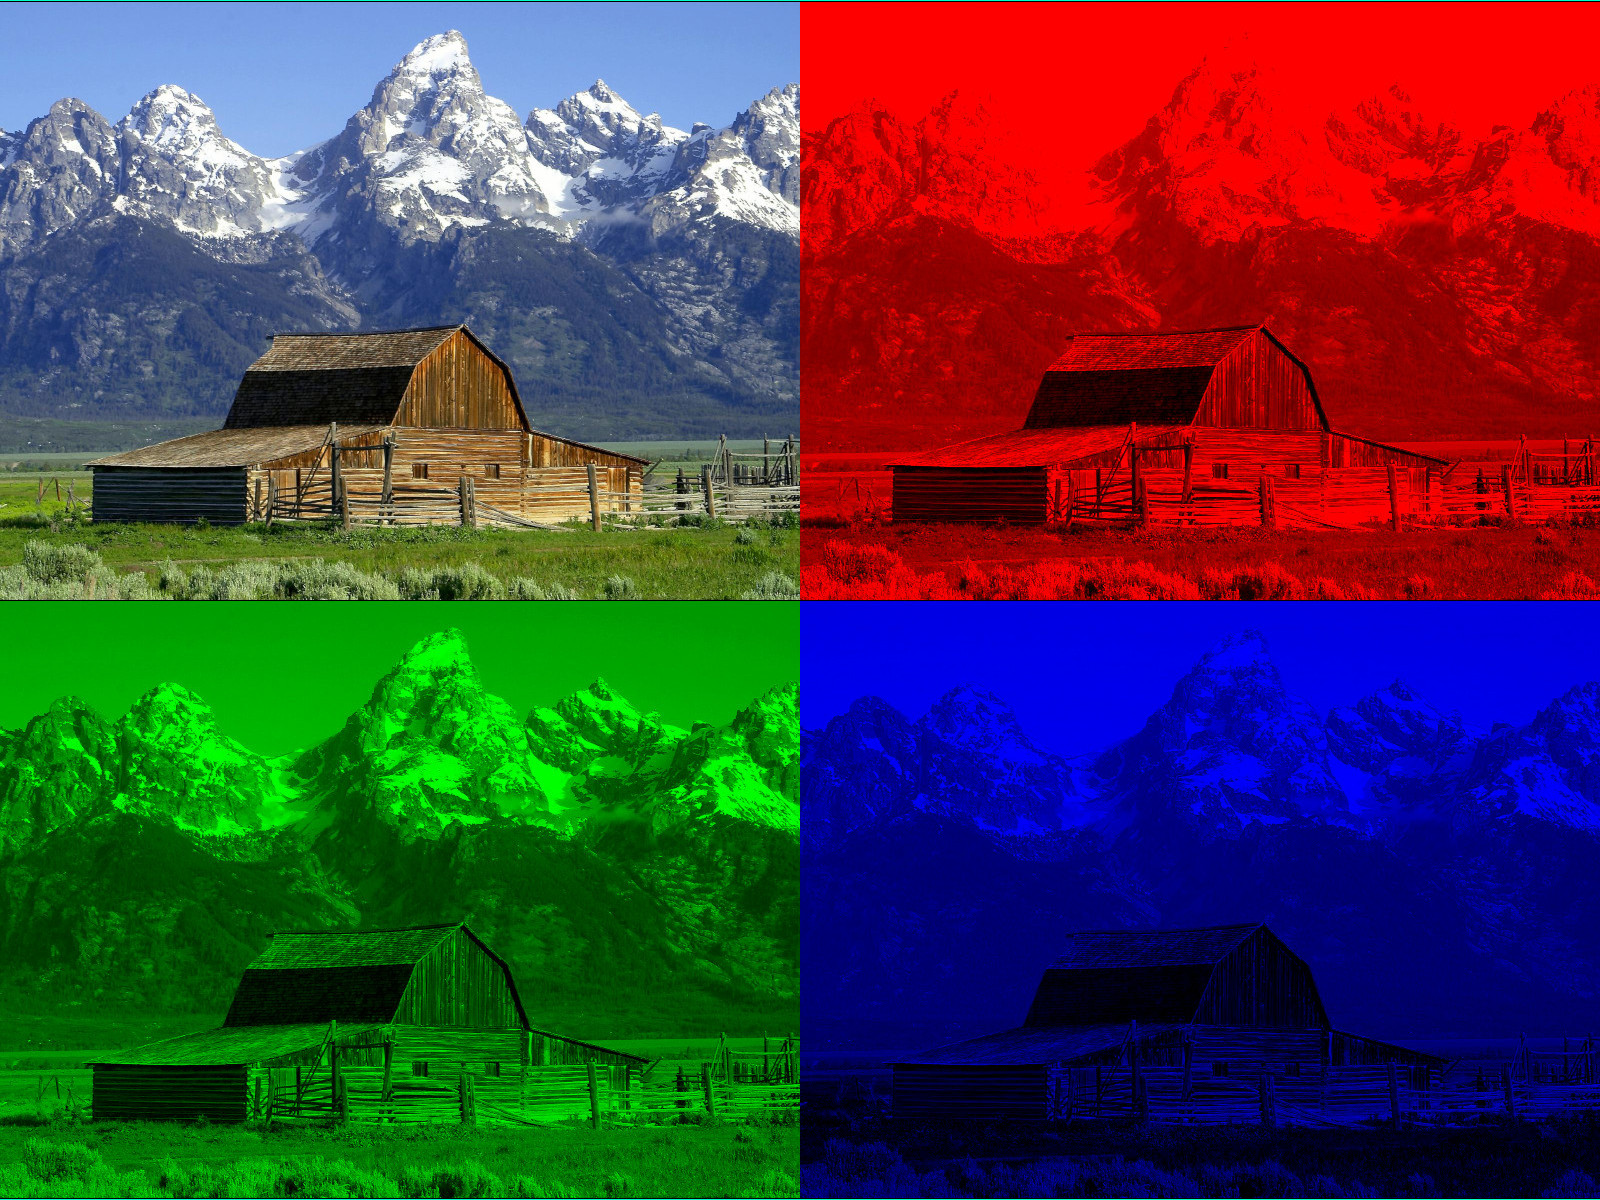
\includegraphics[scale=0.5]{imgs/house-rgbdecomp}
  \caption{An image decomposed into the \emph{R}, \emph{G} and \emph{B} channels
           as used in the \emph{RGB} color model.}
  \label{fig:house-rgbdecomp}
\end{figure}

\begin{figure}[h]
  \centering
  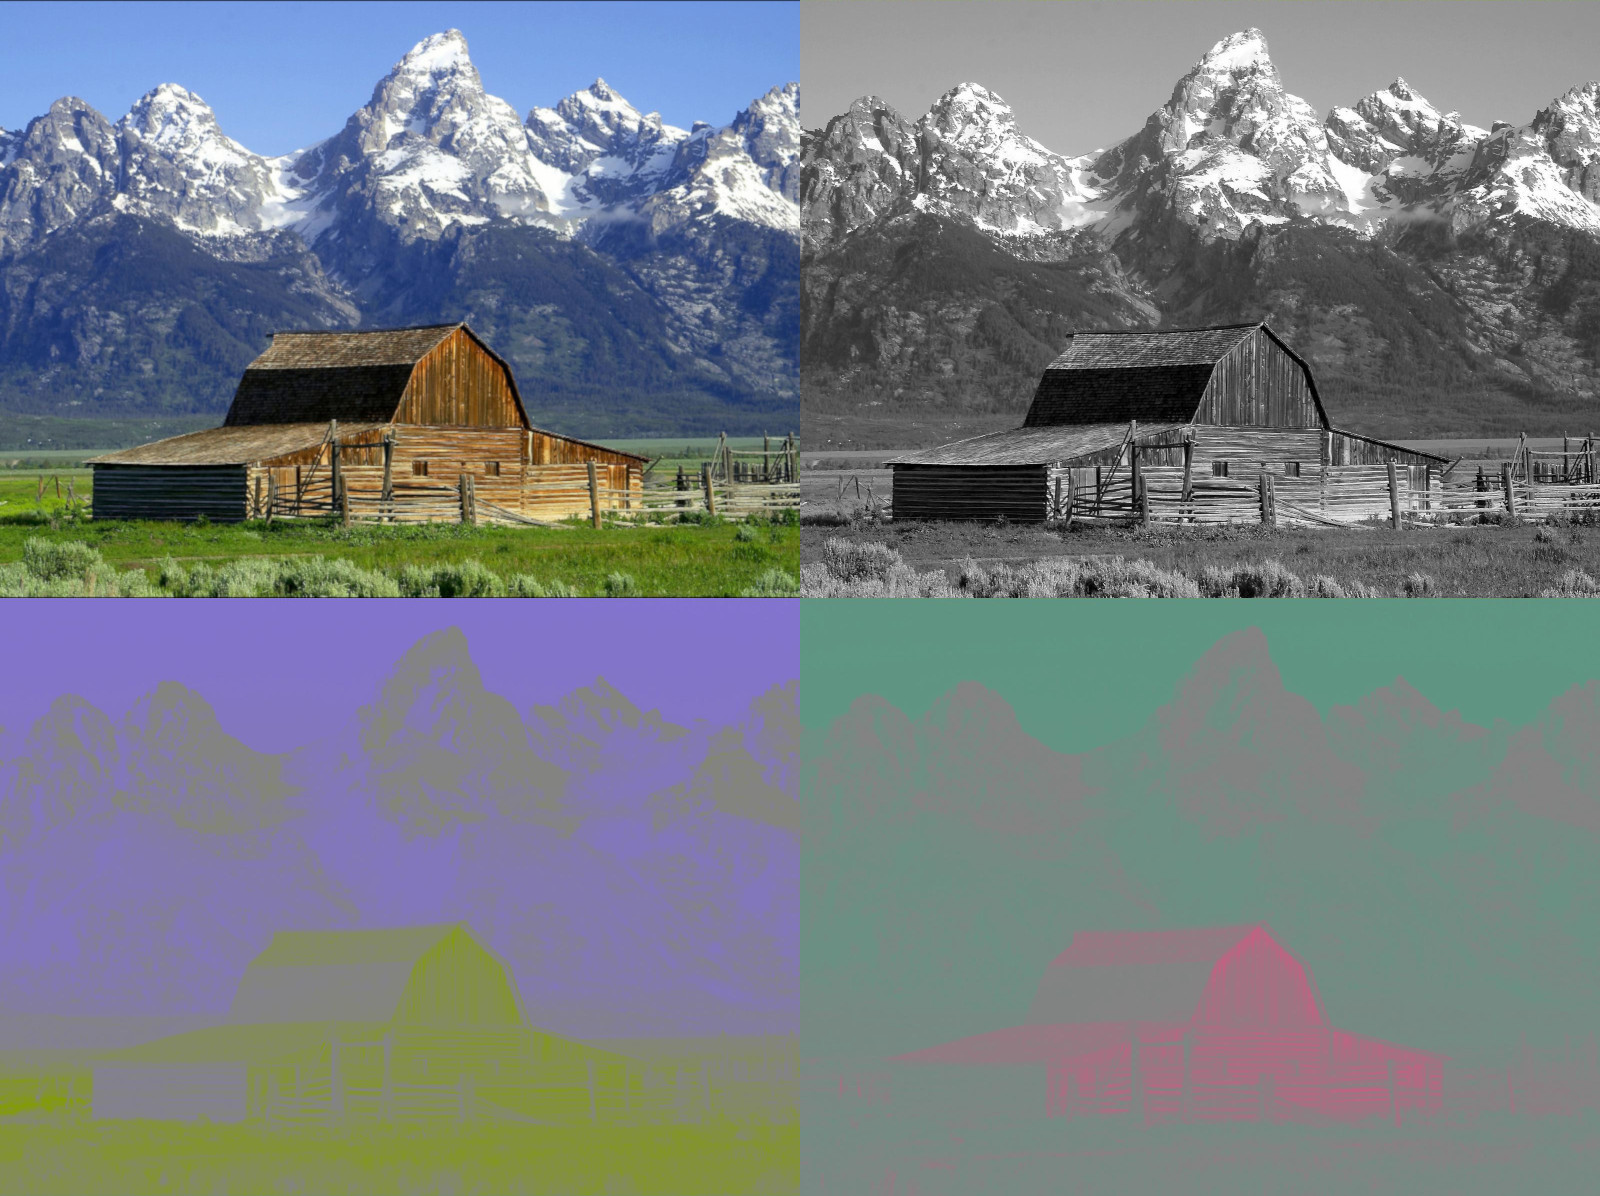
\includegraphics[scale=0.5]{imgs/houses-decomp-ycbcr}
  \caption{An image decomposed into the $Y'$, $C_B$ and $C_R$ components, as used
           in the $Y'C_BC_R$ color space. The $Y'$ component also represents the
           grayscale image.}
  \label{fig:house-ycbcrdecomp}
\end{figure}


\chapter{Image compression}
\label{ch:image-compression}
As it has been shown in the introduction of this thesis, storing uncompressed
images requires a lot of space. The art of reducing the amount of space required
for storing data by encoding information with less bits than would otherwise
be necessary is called data compression.
\\

This chapter will explore the basics of data compression in order to build
a framework for the rest of this thesis. Image compression basics with examples
of current algorithms used for image compression will be described. The end of
the chapter will explore compression metrics which can be used for determining
quality of data compression (as well as image compression).


%http://rahilshaikh.weebly.com/uploads/1/1/6/3/11635894/data_compression.pdf
% Pridat sekci o redundancies
% Taky bych pak mohl napsat sekci o nejaky kompresni srande, co zvolim
\section{Data compression}
When the terms \emph{compression algorithm} or \emph{compression technique} are
used, they refer to two algorithms. One algorithm which takes an input $X$ and
generates a representation $Y$, which requires fewer bits to store. The second
algorithm is the reconstruction algorithm, which operates on the representation
$Y$ and generates the reconstruction $Z$. Depending on whether the reconstruction
$Z$ is completely identical to the original data source $X$, the compression
algorithms can be divided into two broad classes, being either \emph{lossless
algorithms} or \emph{lossy algorithms}. Lossy algorithms generally provide
much higher compression than lossless algorithms do, but at the cost of
losing information.\cite{datacompression}


\subsection{Lossless algorithms}
Lossless compression techniques involve no loss of information - by using
a lossless algorithm, the original data can be recovered exactly from the
compressed data. The applications for lossless algorithms commonly include
text data, where small differences could easily result in wrong statements
(errors in e.g. bank records are, for obvious reasons, very undesirable).


\subsection{Lossy algorithms}
However, not all usage scenarios require compression to be lossless. In
these cases, the requirement of retrieving absolutely identical data can
be relaxed. By relaxing this requirement, very often higher compression
ratios (more on compression ratio in section \ref{metrics}) can be obtained,
at the cost of having distortions in the reconstruction.
\\

Very common scenarios where lossy compression algorithms become often more
desirable than lossless ones are when storing audio content. Modern audio
compression algorithms are almost all lossy - the often used \emph{MP3}
format used for storing audio stores audio with a lossy compression
algorithm. As long as audio is stored without audible artifacts (distortions
which are not present in the original data), the quality of sound does not
have to be perfect - especially when compressing speech. When compressing
other forms of audio, such as music, the compression needs to be more accurate,
but still does not have to be absolutely perfect - as long as the listener
does not notice the difference.
\\

Other typical use case for a lossy compression algorithm is compressing images
or video content. Small distortions are acceptable in images and video as long
as they are not easily noticable by the human eye. However, this can also depend
on the use case - for example photos commonly taken can be compressed in a lossy
way, but medical images often have to be compressed in a lossless way, as artifacts
can be very undesirable for medical usage.

\begin{figure}[h]
  \centering
  
\includegraphics{imgs/sampletext-comparison}
  \caption{A sample image showing how accurate a lossy algorithm can be. The left image
           has been compressed using a lossless algorithm, the right image has been
           compressed using a lossy algorithm (JFIF/JPEG). In this case, essentially
           no artifact can be seen unless zoomed in (as seen in the figure \ref{fig:jfifartifact}).}
  \label{fig:jfifvspng-sample}
\end{figure}

\begin{figure}[h]
  \centering
  
\includegraphics[scale=0.3]{imgs/text-artifacts}
  \caption{A zoomed in image used in the figure \ref{fig:jfifvspng-sample}. While
           almost impossible to notice any artifact in the former example,
           the artifacts can be seen on the borders between the text and the
           gray background easily once zoomed in. Color levels were adjusted
           in order to emphasize the presence of artifacts.}
  \label{fig:jfifartifact}
\end{figure}


\subsection{Modeling and coding}
One of the important factors when designing a compression scheme which needs to
be accounted for are characteristics of data which is to be compressed. An approach
which works the best will depend to a large extent on the redundancies (more on
redundancies in section \ref{sec:imgcmpr-redund}) inherent to the data compressed.
\\

In the phase of modeling, information about any redundancy is extracted in a form
of a model, which can then be utilized in the compression algorithm. The second phase
important in a compression scheme is \emph{coding}. A description of model and how
data differs from the model can be encoded (usually using a binary alphabet).\cite{datacompression}
\\

A very simple example of modeling and coding and its importance can be seen on \emph{delta
encoding} (sometimes also called \emph{delta compression}). Delta encoding encodes
a sequence of messages not by their values but by calculating the difference
between two elements.\cite{signalprocessing} Thus, a sequence such as
\begin{align*}
  10000, 10002, 10001, 99999, 10000
\end{align*}
can be modelled as a sequence where the numbers have very small differences.
When shown as a sequence of differences, with the original value, the sequence
then becomes:
\begin{align*}
  10000, +2, -1, -2, +1
\end{align*}
\\

After a representation of this data sequence has been modeled, the coding phase
creates a way how to encode this sequence using this model. One possible
coding is shown in the table \ref{tab:deltacoding}. Utilizing this coding, the
differences require only 2 bits in order to be stored.
\\

\begin{table}[]
\centering
\begin{tabular}{|l|l|}
\hline
+1 & 00 \\ \hline
+2 & 01 \\ \hline
-1 & 11 \\ \hline
-2 & 11 \\ \hline
\end{tabular}
\caption{Example coding for a sample data sequence using delta encoding}
\label{tab:deltacoding}
\end{table}

However, delta encoding would not be efficient in a scenario when
the data has large differences - especially if the differences would be larger
than storing the data itself. Understanding the type of data when creating a model
is therefore highly important.


\section{Image compression}
Commonly, data compression algorithms are discussed as universal techniques
which are able to compress essentially any data. While these algorithms might still
have preferred applications, literature commonly separates techniques from the applications.
However, image compression is a specific field where separating techniques from
the application is essentially impossible as the techniques are meant specifically
for compressing images.\cite{datacompression}
\\

While compressing image data using standard compression techniques, none of them
are satisfactory for color or grayscale images (which were discussed in chapter
\ref{ch:image-encoding}). For example, statistical methods can be very good for
compressing data where each value has different probability (such as in standard
text, where certain letters appear far less than others). However, in images, certain
colors or shades of gray often have the same probabilities.\cite{datacompressioncompleteref}
\\


% TODO obrazek, ktery ukazuje redundance na 3 obrazcich
\subsection{Redundancies in images}
\label{sec:imgcmpr-redund}
In order to understand how image compression techniques work, certain aspects of
images need to be characterized, as compression techniques try to use these
aspects for their advantage. A fundamental component of image compression is
reducing the amount of redundancies present in the signal source. The redundancies
commonly present in images are these ones:

% src pro popis - fromdcttowavelet
\begin{itemize}
  \item Coding redundancy
  \item Interpixel redundancy (also sometimes spatial redundancy)
  \item Psychovisual redundancy
\end{itemize}
\cite{fromdcttowavelet}

\emph{Coding redundancy} occurs when length of the code words is larger than
required. A simple example of coding redundancy can be shown on a grayscale
image where only certain shades of gray are used. Instead of requiring
8 bits per shade of gray, such an image might require far less bits to
encode, as can be seen on \ref{img:redundancies}.
\\

\emph{Interpixel redundancy} refers to the fact that usually, neighbouring pixels
tend to have similar colors. Therefore, it can often be possible to predict
the color of neighbouring pixels. As a simple example, black-and-white images
might be encoded using \emph{run-length encoding}, where instead of 
encoding the specific colors per pixel, an information about how many
pixels of the same color are stored in a row. This can be particularly
efficient when considering bi-level (black-and-white) images, as can be seen
on \ref{img:redundancies}.
\\

The last kind of redundancy which is commonly utilized in image compression
algorithms is called \emph{psychovisual redundancy}. The human eye is not
able to perceive certain visual information in an image - such information could
be discarded without any noticeable artifacts present in the compressed image.
A tool commonly used for reducing psychovisual redundancies in an image is
\emph{discrete cosine transform}, which is also used in the JFIF/JPEG image
format.

\begin{figure}[h]
  \centering
  
\includegraphics{imgs/redundancies}
  \caption{A sample image showing some of the redundancies which can be present in an image.
  		  As there are only 4 levels of gray color, storing them using 8 bits
  		  per possible gray color would result in high coding redundancy. Also,
  		  neighbouring pixels almost always have the same colors.}
  \label{fig:redundancies}
\end{figure}

% potencialni todo - extendovat psnr/mse o vysvetleni, jak se pocitaji s barvickama
% [TODO] obrazek, ktery ukazuje mse a psnr
\subsection{Compression metrics}
\label{metrics}
%lossy, lossless, compression ratia jpg png ...
When evaluating the quality of a compression technique, utilizing certain
metrics is necessary - especially when attempting to compare compression
algorithms.
\\

One of the most important metrics is the \emph{compression ratio}.
Compression ratio is a very simple metric which quantifies the reduction
in data representation needed. It can be easily defined in the following
way:
\begin{equation}
Compression\ Ratio = \frac{Uncompressed\ size}{Compressed\ size}    
\end{equation}

It is easy to see that compression ratio is an essential metric as
it makes it very easy to compare compression algorithms or even
quantify their compression power in general. Certain metrics
extend compression ratio and use it for scoring purposes, such as
the \emph{Weissman score} which can be used for lossless compression
algorithms. \cite{CITATIONNEEDED}.
\\

However, while compression ratio is a very valuable metric and
highly valuable for lossless algorithms, it potentially stops
being the most important metric when evaluating lossy algorithms.
When evaluating lossy algorithms, the important information is not
only quantification of how much was the data compressed but also
evaluating how much information was actually lost in the compression
process. As an example, if a lossy algorithm has better compression
ratio than another one, it might still not be the algorithm of choice,
in the case where it would introduce too many artifacts into the data.
\\

%[TODO] citation: http://www.debugmode.com/imagecmp/index.htm
Thus, it is necessary to introduce other compression metrics, which
can be utilized for evaluating the performance of lossy compression
algorithms, related to information loss - or in other words, the errors
present in data after reconstruction. The two error metrics which are
commonly used when measuring the performance of a lossy compression
algorithm are the \emph{mean squared error} (MSE) and \emph{peak
signal-to-noise ratio} (PSNR).\cite{imgcomprintro}
\\

Mean squared error is a statistical metric measuring the average
of the squared of errors (the difference between original values and
the values after decompressing data and obtaining the reconstruction).
When used for image compression, the metric can be formalized in the
following way:
\begin{equation}
    MSE = \frac{1}{MN}\sum_{y=1}^{M}\sum_{x=1}^{N}(I(x,y) - I'(x,y))^2
\end{equation}
where
\begin{itemize}
    \item $M$ and $N$ are the dimensions of an image
    \item $I(x, y)$ is the value of a pixel on coordinates $x, y$ in the
    original image.
    \item $I'(x, y)$ is the value of a pixel on coordinates $x, y$ in the
    reconstructed image.
\end{itemize}
A lower value of MSE is better, as it directly displays less errors present
in the decompressed image.
\\

Peak signal-to-noise ratio is a metric derived from MSE describing the ratio
between the maximum possible power of a signal and the power of corrupting
noise which affects the representation. Due to signals possibly having
a very wide dynamic range, PSNR is usually expressed in the logarithmic scale.
\\

With MSE defined as above, PSNR can be formalized as:
\begin{equation}
    PSNR = 20 \cdot log10 \left( \frac{MAX^2_I}{MSE} \right)
\end{equation}
where $MAX_I$ is the maximum possible value of a pixel in an image. In the
case of grayscale images stored with 8 bits per pixel, this value would
be 255. Unlike MSE, higher PSNR values are better, as they are a sign of less errors
in data - signal being the original colors and noise being errors.
\\

When evaluating MSE (and consecutively PSNR) for color images, the calculation becomes
slightly more difficult, as a pixel value of I[x, y] holds multiple values for multiple
components, which are all perceived differently by the human eye. Some of possible approaches
can therefore be the following:
\begin{itemize}
  \item Evaluate MSE and PSNR for each component. Resulting MSE (or PSNR respectively)
  is the average of MSE values of each component (or PSNR values of each component, 
  respectively).
  \item Due to brightness being the most important element for human eye, rather than
  color components, evaluate MSE and PSNR values only of luma (or simply the grayscale
  image). The definition of luma as a weighted sum has been explored in chapter \ref{ch:image-encoding}.
\end{itemize}
\cite{matlab18}\cite{netpbm}

%[TODO] citace - viz wiki psnr
However, it needs to be noted that PSNR is not a perfect metric in the sense
that it would provide absolute definite conclusions. When utilizing PSNR, it is
still important to also consider data subjectively, as it is only conclusively
valid in scenarios where the compared results come from the same codec (or codec
type) and the same content. Not only that, but it is a metric which is not
performing strongly as a quality metric when it comes to human perception
of image data. \cite{psnrsucks1} \cite{psnrsucks2} Still, it is a metric often
utilized to evaluate lossy compression
of images.
\\

%[TODO] better wording
Last but not least, one of the important metrics, just like when
evaluating performance of any other algorithm, is the required
time to execute the compression algorithm (as well as decompression
time).

\subsection{JPEG image compression}
As noted in chapter \ref{ch:NMF}, non-negative matrix factorization can
be understood as a lossy compression algorithm - approximating the
data in an original matrix by two smaller matrices which have less
elements in total than the original matrix. As this process necessarily
involves data loss (as non-negative matrix factorization solves the problem
of approximating the original matrix, not finding an exact representation),
a compression algorithm based on non-negative matrix factorization has to be
a lossy one. Thus, the image compression algorithms which are going to be
discussed in this thesis are lossy ones. Also, as this thesis is related
to creating a proof of concept image compression scheme based on non-negative
matrix factorization and not describing all the existing lossy image
compression schemes, only the JPEG compression scheme will be explored,
as the results of the \emph{NMF} compression scheme will be compared to
JPEG.
\\

The JPEG compression method is commonly used for compressing digital
photographies and makes it possible to adjust the degree of compression
- making it possible to decide the tradeoff between image quality and
compression. Commonly, JPEG is able to achieve 10:1 compression ratio
without significant perceptible loss in image quality.\cite{jpegcompression}
\\

The JPEG compression algorithm can use various modes of operation, but
the most popular one works in the following way:
\begin{itemize}
    \item An image is converted from $RGB$ to $Y'C_BC_R$.
    \item The resolution of chroma is reduced - this is done as the human eye is less
    sensitive to color details than brightness.
    \item The image is split into $8 \times 8$ pixel blocks. For each component of $Y'C_BC_R$
    the 8x8 block is transformed using the discrete cosine transform. By doing so,
    the image data is represented in the frequency domain.
    \item The amplitudes of the frequencies are quantized, meaning that components
    with high frequencies are stored with less accuracy than the ones with lower
    frequencies.
    \item The resulting data of $8 \times 8$ blocks is further compressed using lossless
    encoding.
\end{itemize}
These steps are all able to reduce all three redundancies presented in the previous
sections - psychovisual redundancies are removed by storing higher frequencies with
lower accuracy and interpixel redundancy by working no $8 \times 8$ pixel blocks. Coding
redundancy is reduced using a lossless compression algorithm at the end.

% [NTH] mozna napsat kapitolu, ktera ukaze schopnost JPEG komprese na nejakych metrikach,
% ale je to soucast porovnavani vuci mymu algoritmu, tak uvidime.


%Vlastnosti NMF popsane
%  - neunikatnost NMF - muze byt rozdilna velikost se stejnou kvalitou (i kdyby se dosahlo perfekce, muze byt vice reseni, to je pak slovnikove komprimovano)
%  - NMF posilano jen na chromu v ycbcr
\chapter{NMF compression scheme}

The previous three chapters all explored the essentials required to construct an image
compression scheme based on non-negative matrix factorization. Utilizing these concepts,
proof of concept compression schemes will be designed in this chapter. The following
implementation is described in the following chapter \ref{ch:implementation}.


\section{Compression scheme design}
As it has been shown in chapter \ref{ch:NMF}, non-negative matrix factorization
can be understood as a lossy compression scheme for matrices, as the original
matrix can be approximated by factor matrices which possibly require less
space to store. However, as there are multiple ways of representing and encoding
an image with different tradeoffs, two compression schemes will be constructed
and compared with each other - a naive one and a scheme based on compressing
chroma values.


\subsection{NMF properties}
However, before the compression schemes are designed, there are some features
of non-negative matrix factorization which should be noted here, as understanding
the effects and limitations of non-negative matrix factorization is important for
constructing these schemes. These properties are the following:
\begin{itemize}
  \item Optimization problem - takes pretty long
\end{itemize}


\subsection{Naive compression scheme}
fgs


\subsection{$Y'C_BC_R$ compression scheme}
fds


\chapter{Implementation}
\label{ch:implementation}
fgsfds


\setsecnumdepth{part}
\chapter{Conclusion}


\bibliographystyle{iso690}
\bibliography{mybibliographyfile}

\setsecnumdepth{all}
\appendix

\chapter{Acronyms}
% \printglossaries
\begin{description}
  \item[NMF] Non-negative matrix factorization
  \item[PNG] Portable Network Graphics
  \item[JPEG]
  \item[PCA] Principal Component Analysis
  \item[SVD] Singular Value Decomposition
\end{description}


\chapter{Contents of enclosed CD}

%change appropriately

\begin{figure}
	\dirtree{%
		.1 readme.txt\DTcomment{the file with CD contents description}.
		.1 exe\DTcomment{the directory with executables}.
		.1 src\DTcomment{the directory of source codes}.
		.2 wbdcm\DTcomment{implementation sources}.
		.2 thesis\DTcomment{the directory of \LaTeX{} source codes of the thesis}.
		.1 text\DTcomment{the thesis text directory}.
		.2 thesis.pdf\DTcomment{the thesis text in PDF format}.
		.2 thesis.ps\DTcomment{the thesis text in PS format}.
	}
\end{figure}

\end{document}
